\begin{figure}[htb]
\centering
 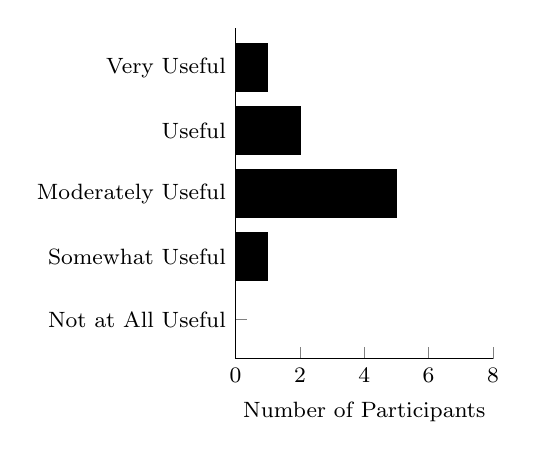
\begin{tikzpicture}
 \begin{axis}[
     xbar stacked,
     ytick=data,
     axis y line*=none,
    axis x line*=bottom,
    tick label style={font=\footnotesize},
    legend style={font=\footnotesize},
    label style={font=\footnotesize},
    xtick={0,2,4,6,8},
    width=.4\textwidth,
    bar width=6mm,
    xlabel= Number of Participants,
    yticklabels={Not at All Useful, Somewhat Useful, Moderately Useful, Useful, Very Useful},
    xmin=0,
    xmax=8,
    area legend,
    y=8mm,
    enlarge y limits={abs=0.625},
]

\addplot[fill=black] coordinates
{(0,0) (1,1) (5,2) (2,3) (1,4)};
\end{axis}  
\end{tikzpicture}
\caption{Survey Results on the Usefulness of \tooltwo}
\label{fig:class-survey}
\end{figure}